\section{Messergebnisse und Auswertung}
\subsection{Peltierelement}

\begin{figure}[H]
\begin{center}
  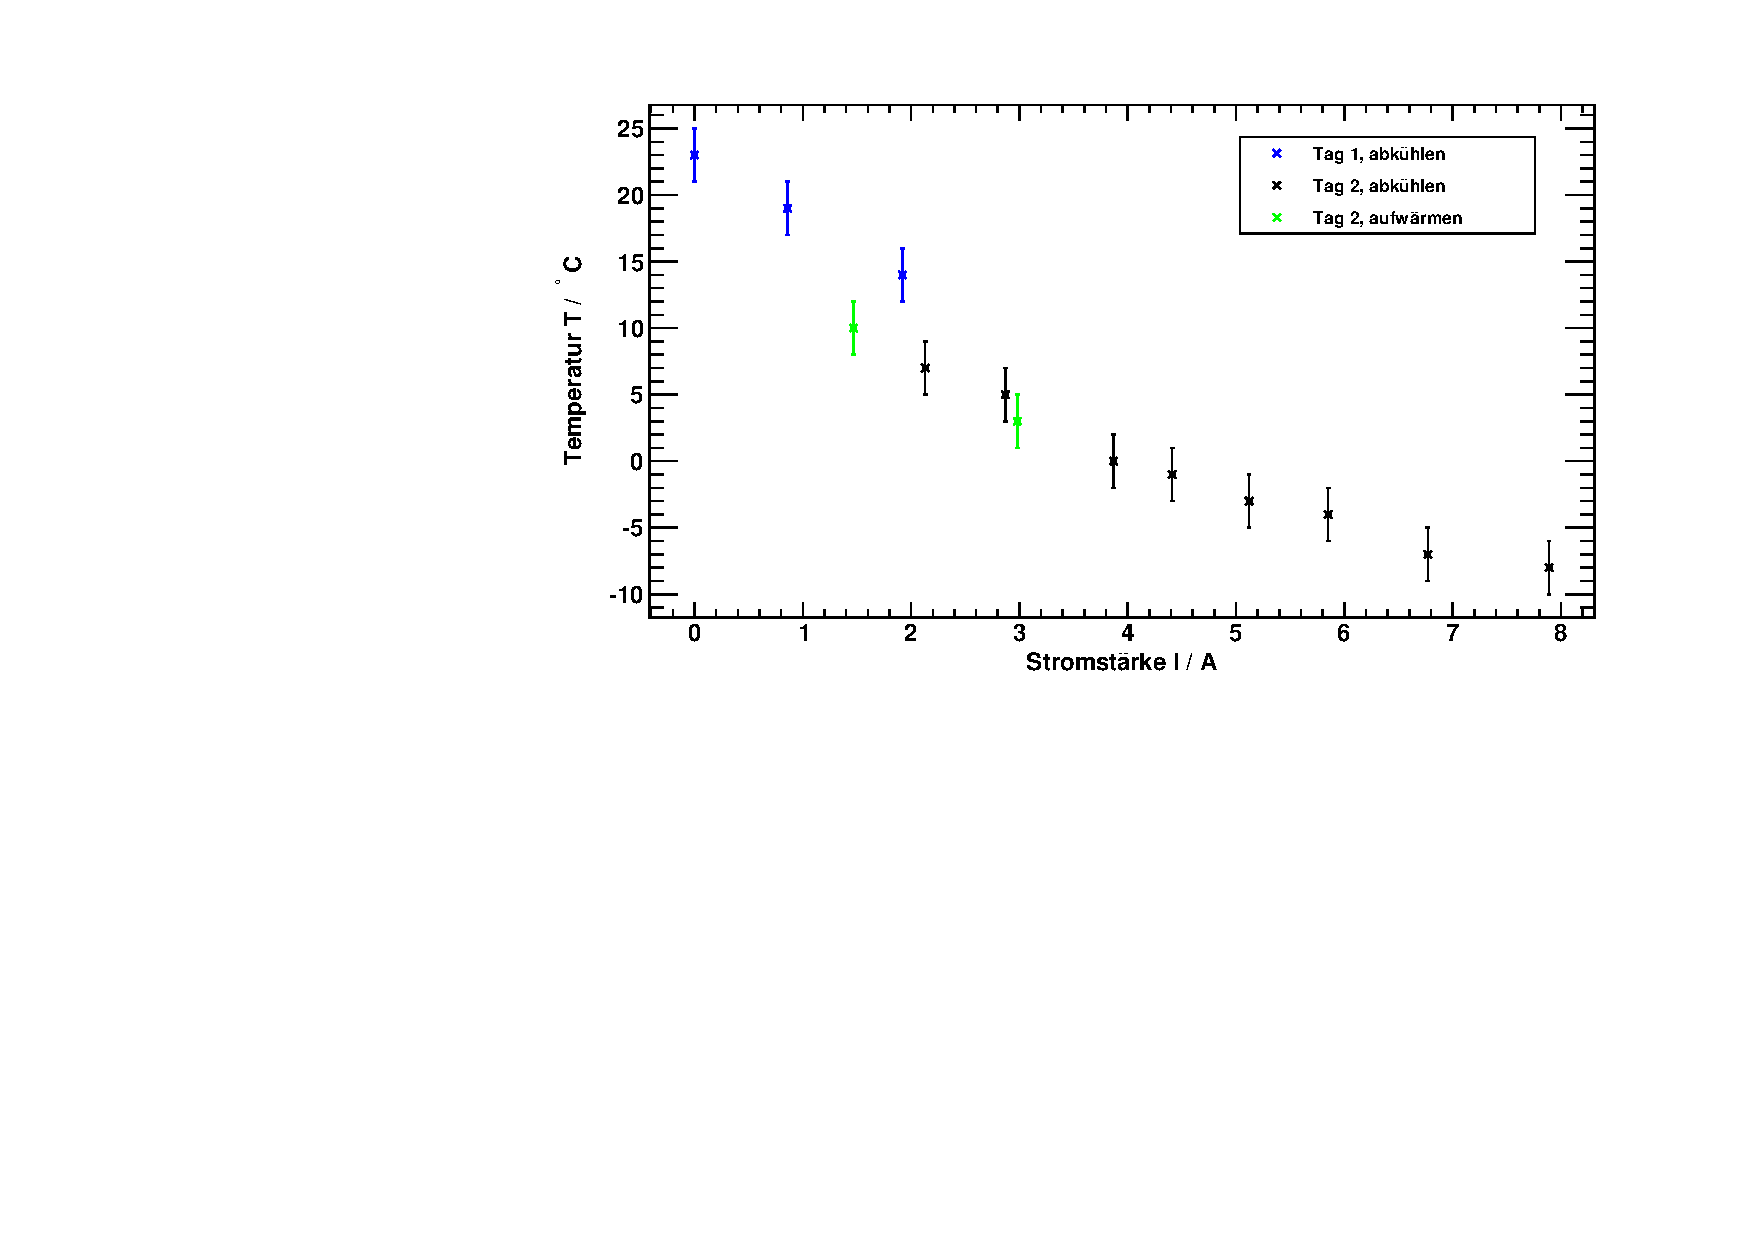
\includegraphics[width=\textwidth]{../img/graph_T-I.pdf}
  \caption{Temperatur am Thermoelement
  in Abhängigkeit des Stroms durch das Peltierelement.}
  \label{img:TI}
\end{center}
\end{figure}

\autoref{img:TI} zeigt den Zusammenhang zwischen Strom durch das Peltierelement
und der Temperatur, die sich nach 30 Minuten Stromfluss am Thermoelement eingestellt hat.
Es ist ein exponentieller Verlauf mit Sättigung bei hohem Strom zu erkennen.
Dies kann mit dem Wärmefluss aus der Umgebung begründet werden.
Als Fehler auf den Strom wurde hier zwei Digits ($s_I=0.02$\,A) und auf die Temperatur $s_T$=2\,K gewählt.
Auf einen Fit wurde hier verzichtet, da die genaue Information über den Zusammenhang
für die Auswertung nicht relevant ist.
Man erkennt allerdings, dass die Messwerte für Abkühlung (schwarz) und Erwärmung (grün) konsistent sind.
Die Einschwingzeit von 30 Minuten ist also lang genug gewählt.
Zwischen 1. und 2. Messtag besteht ein großer Offset.
Dies könnte an der Temperatur des Kühlwassers liegen,
das am ersten Tag von einem anderen Verbraucher im Haus erwärmt wurde.\\
\autoref{img:UI} zeigt die Strom-Spannungs-Kennlinie des Peltierelements.
Der Fehler auf den Strom ist wie oben und der auf die Spannung ebenfalls zwei Digits ($s_U=0.2$\,V).
Der Zusammenhang ist linear, der Widerstand beträgt über den gesamten Arbeitsbereich ca. 3\,\textOmega.
Die Kühlleistung des Elements ist also sowohl zum Quadrat des Stroms als auch zum Quadrat der Spannung proportional.



\begin{figure}[H]
\begin{center}
  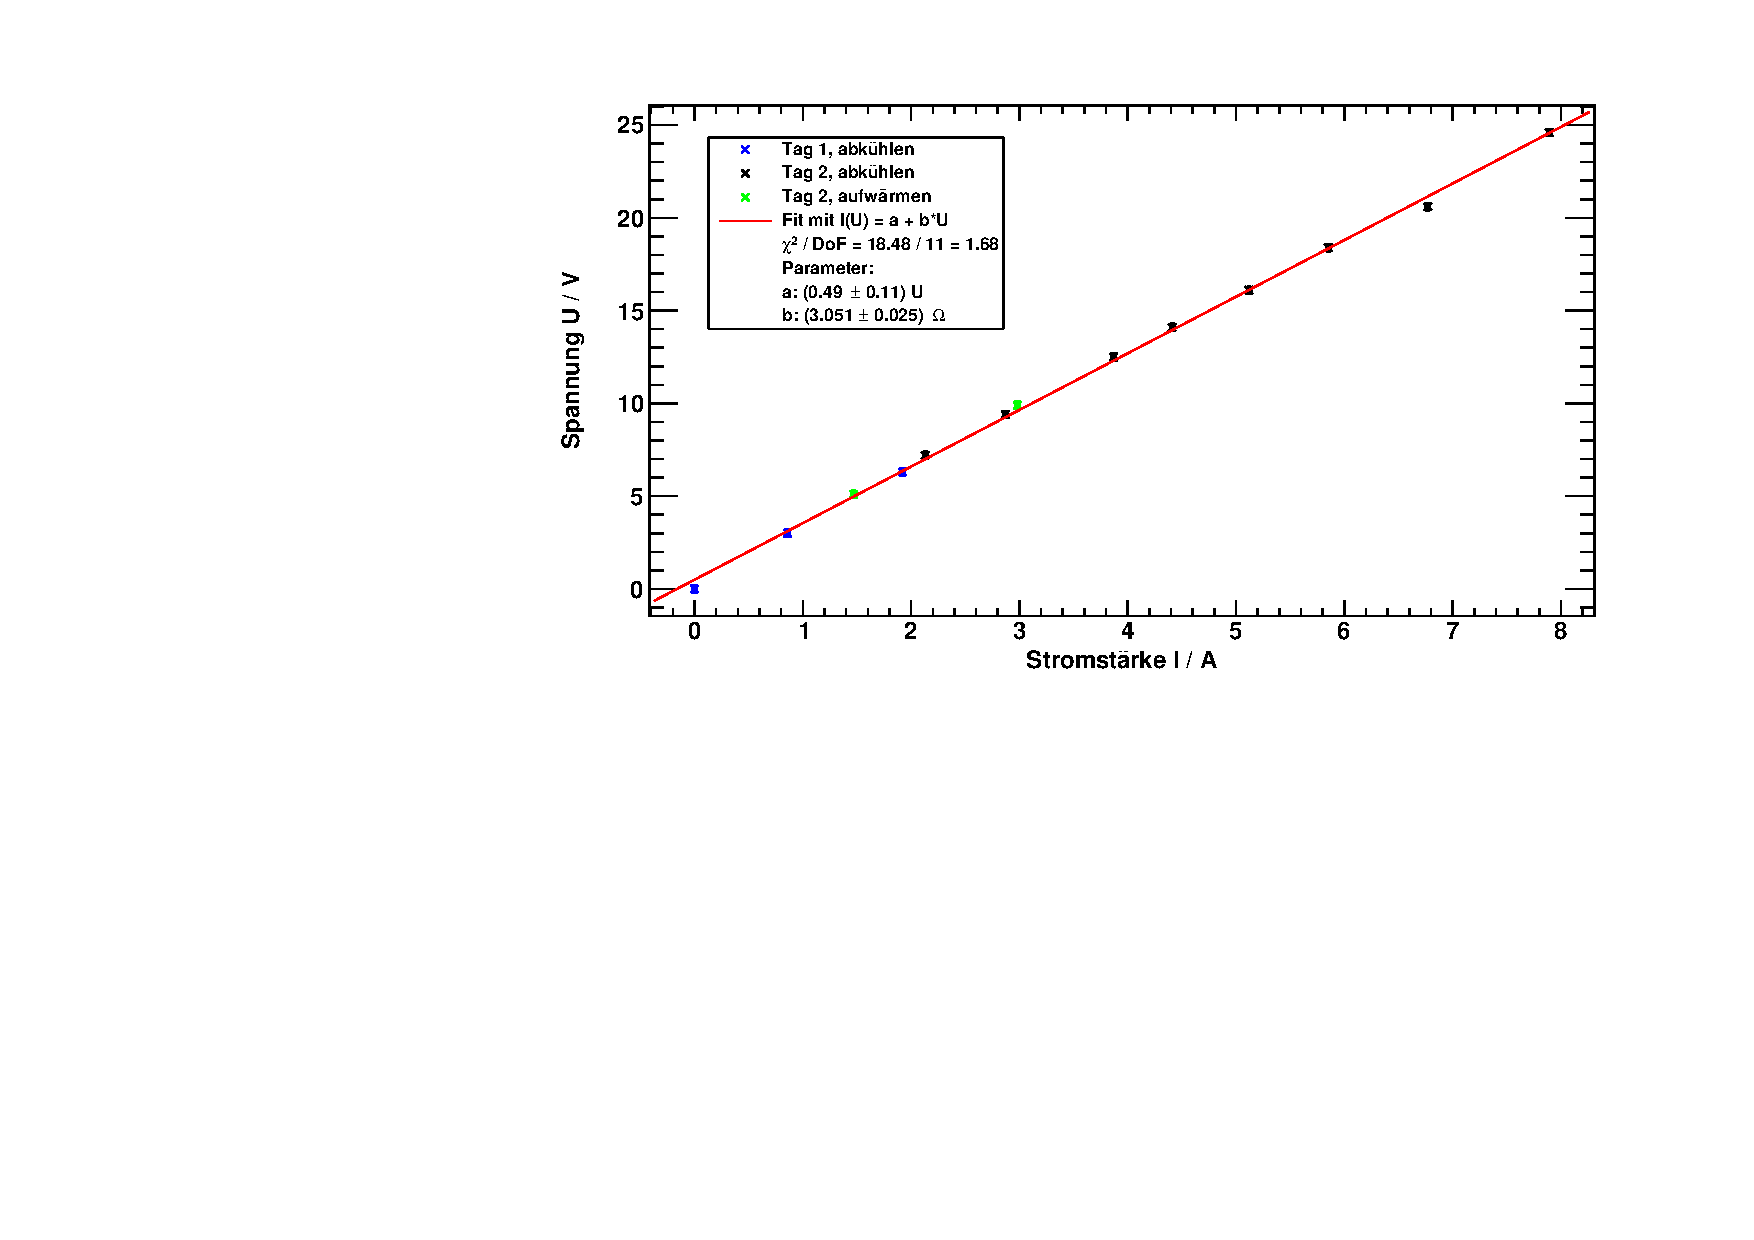
\includegraphics[width=\textwidth]{../img/graph_U-I.pdf}
  \caption{Strom-Spannungs-Kennlinie des Peltierelements.}
  \label{img:UI}
\end{center}
\end{figure}




\subsection{Bestimmung der Lebensdauer aus dem Lorentz-Peak}
\subsubsection{Vorgehensweise}
Für jede Messung erhält man zwei Graphen: Die Abhängigkeit der Rampenspannung $U$, die an der Spule anliegt, von der Zeit und der 
zeitliche Lorentzpeak des Hanle-Effekts. Die Spannung $U$ wird in dem Wertebereich, in dem sie sich verändert, mit 
einem Polynom ersten Grades gefittet (\autoref{img:fit:BV}). Der Fehler auf die Spannung $U$ und die Zeit $t$ wurde jeweils auf die Hälfte der 
Binbreite gesetzt.\footnote{Diese Werte werden hier nicht explizit angegeben, da sie für verschiedene Messungen aufgrund der unterschiedlichen 
Auflösung des Oszilloskops variieren.}
\begin{equation}
  \label{eq:BV:fitfunction}
  U(t) = a + b \cdot t
\end{equation}
\begin{figure}[H]
\begin{center}
  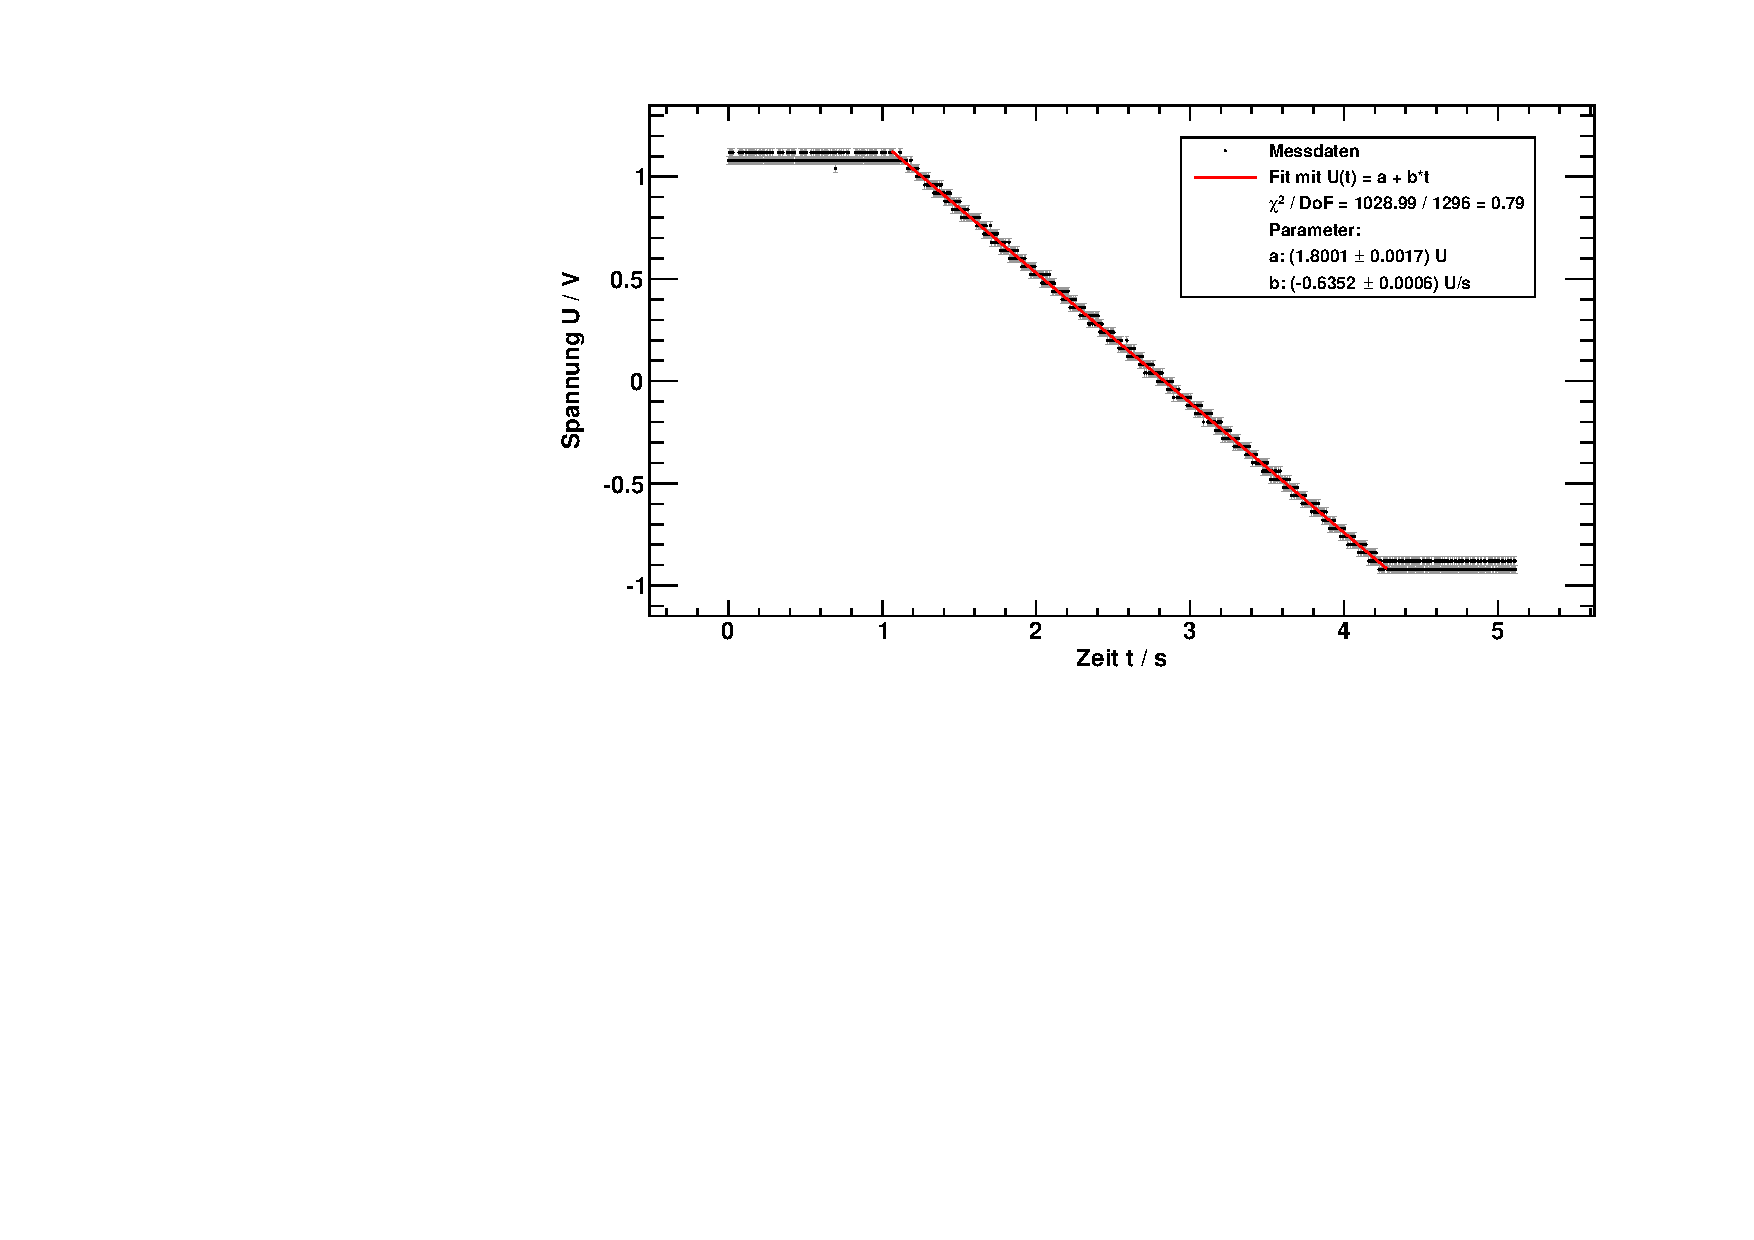
\includegraphics[width=\textwidth]{../img/fitBV_00_m03.pdf}
  \caption{Linearer Fit der angelegten Spannung $U$ an der Spule. Hier exemplarisch für $T=-3\,{}^\circ$C und $\Phi=0^\circ$.}
  \label{img:fit:BV}
\end{center}
\end{figure}
Da sich der Strom $I$, der durch Spule fließt, direkt aus dem Wert der Spannung $U$ ergibt ($I(t) = U(t) \cdot 1\,\frac{\text{A}}{\text{V}}$), kann man nun zu 
jedem Zeitpunkt $t$ (innerhalb der Änderung von $U$) die Stärke $B$ des angelegten Magnetfeldes bestimmen. Dazu benötigt man eine spulenspezifische 
Proportionalitätskonstante $p$, (hier $p=3.363\cdot10^{-4}\,\frac{\text{T}}{\text{A}}$), 
welche die Änderung des Flusses $B$ mit dem Strom $I$ beschreibt. 
Es folgt:
\begin{equation}
  B(t) = p \cdot I(t)
\end{equation}
Daraus lässt sich nun die Intensität des Hanle-Signals in Abhängigkeit des vorhandenen Magnetfeldes $B$ angeben (\autoref{img:fit:lorentz:0}, 
\autoref{img:fit:lorentz:45}, \autoref{img:fit:lorentz:90}).
Der Fehler auf das Magnetfeld wurde zu 1\% des Wertes gewählt. Auf die Intensität (hier gemessene Spannung $U$) wurde zusätzlich zur halben Binbreite 
noch ein relativer Fehler von $s_\text{rel} = 1\%$ des Messwerts gesetzt:\footnote{Begründet mit Intensitätschwankungen des Photomultipliers.}
\begin{equation}
  s_U = \sqrt{s_{\text{Bin}}^2 + (s_\text{rel} \cdot U)^2}
\end{equation}
Dieser Graph kann nun mit \autoref{eq:intensity} gefittet werden; die Lebensdauer kann direkt aus dem Fit abgelesen.
\begin{figure}[H]
\begin{center}
  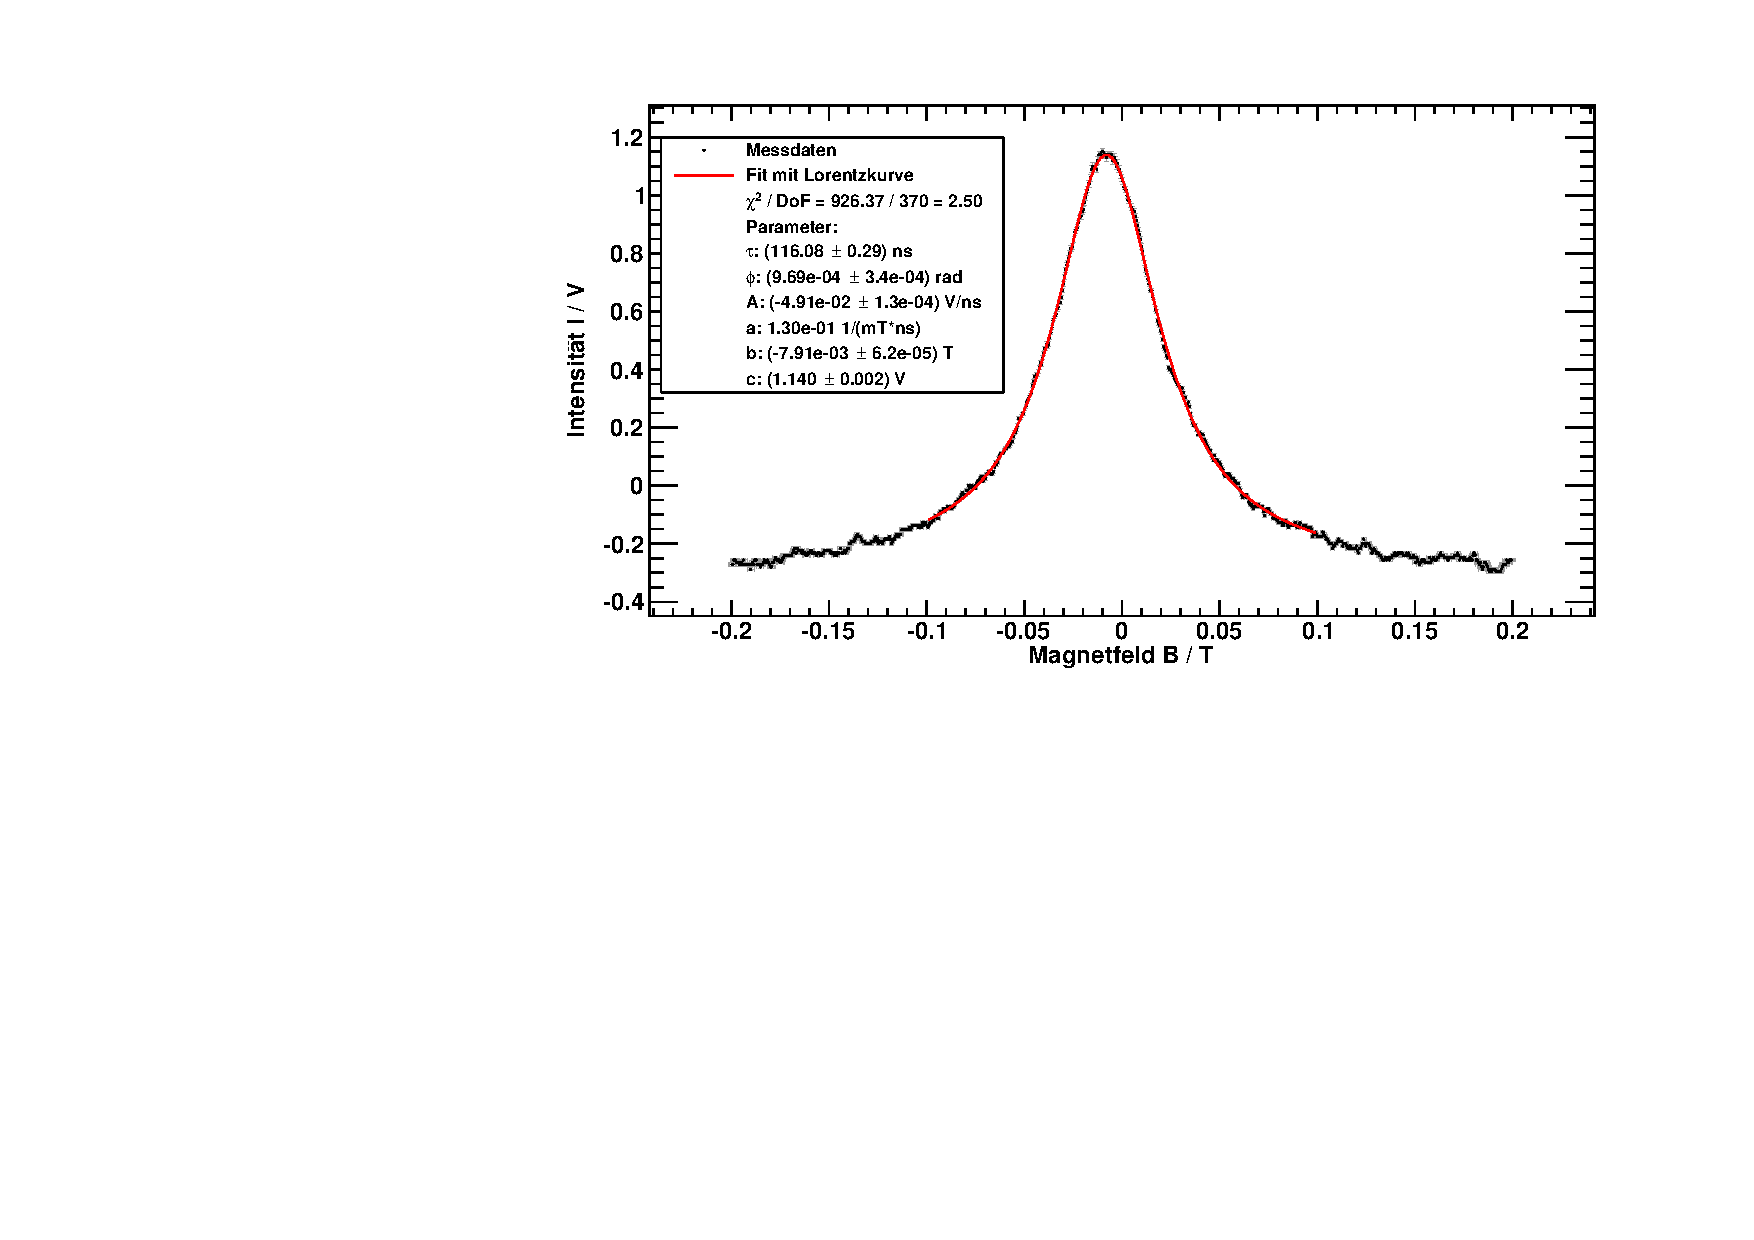
\includegraphics[width=\textwidth]{../img/fit_00_p05_1.pdf}
  \caption{Fit des Hanle-Signals mit Lorentzkurve. Hier exemplarisch für $T=5\,{}^\circ$C und $\Phi=0^\circ$.}
  \label{img:fit:lorentz:0}
\end{center}
\end{figure}
\begin{figure}[H]
\begin{center}
  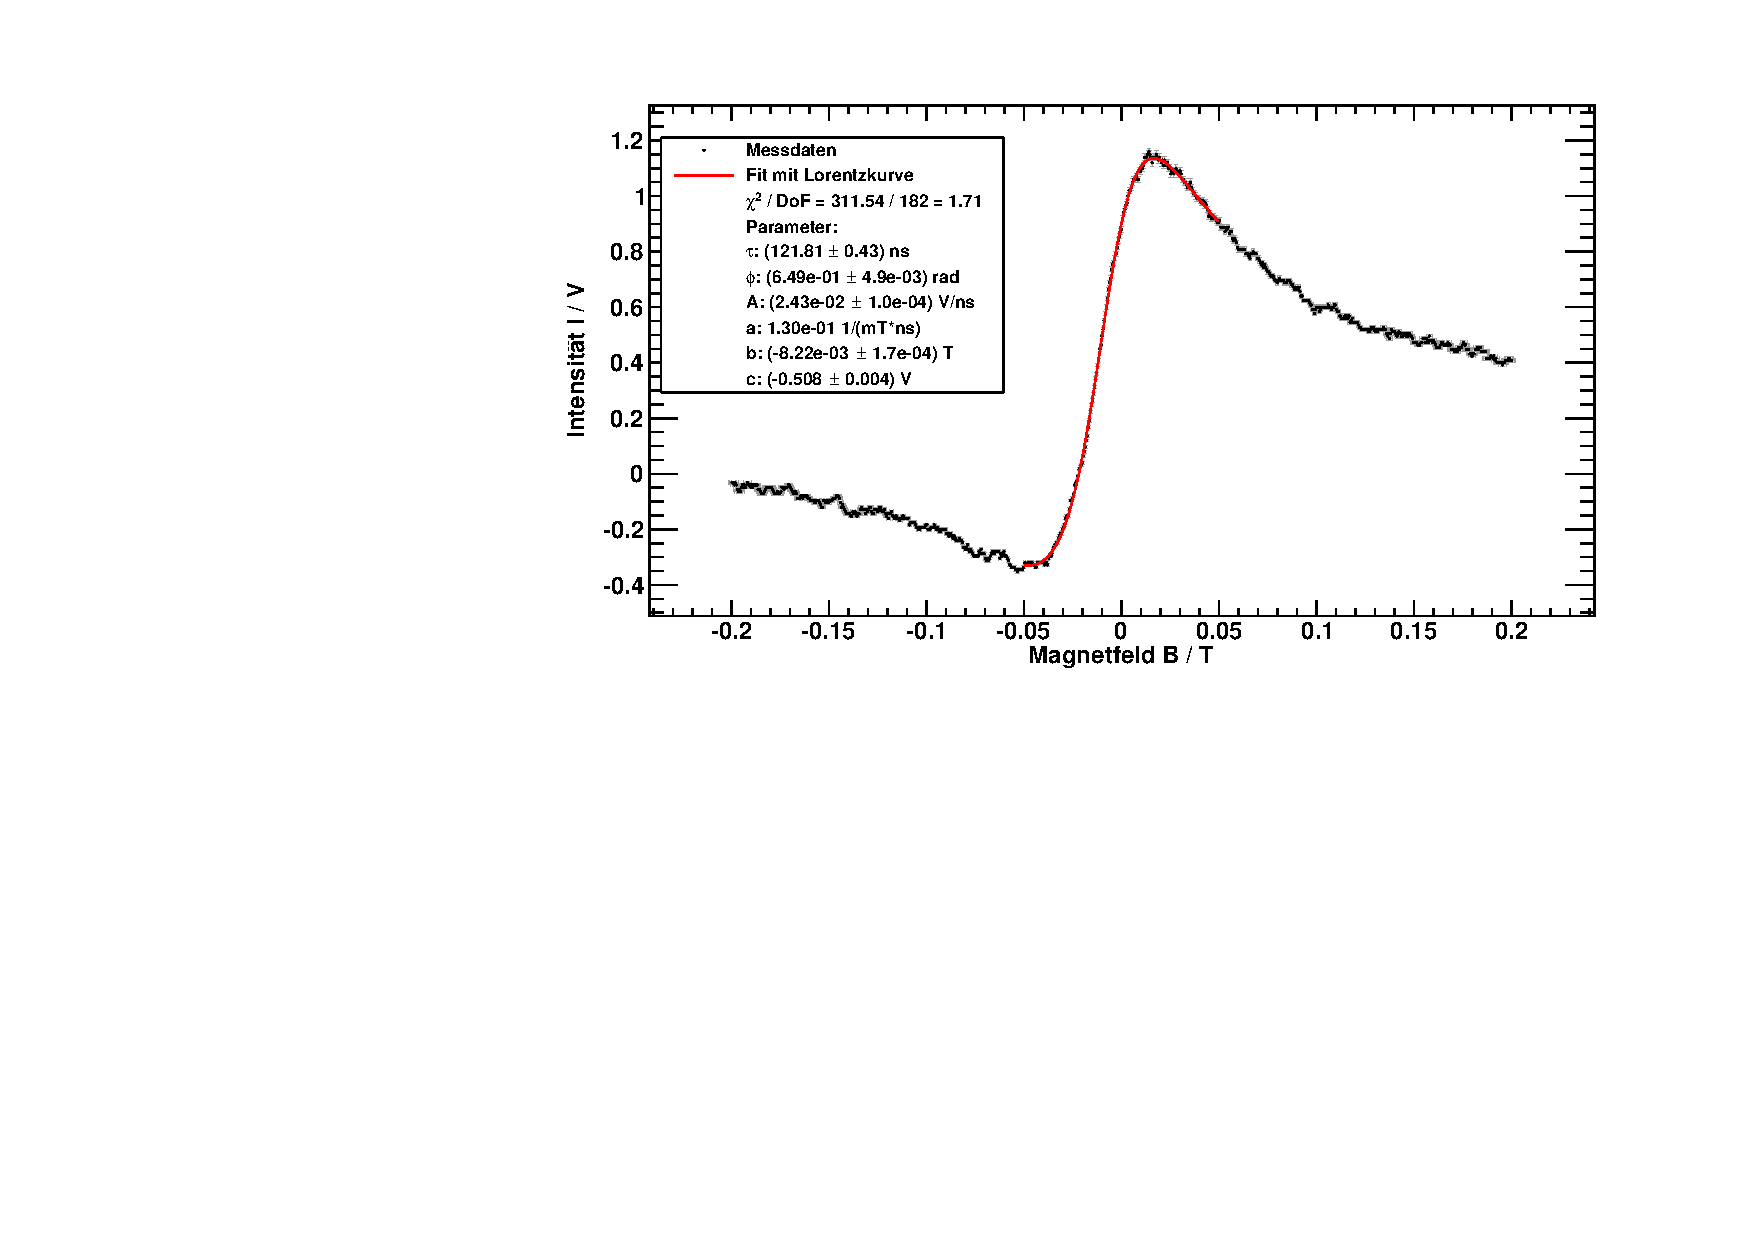
\includegraphics[width=\textwidth]{../img/fit_45_p05.pdf}
  \caption{Fit des Hanle-Signals mit Lorentzkurve. Hier exemplarisch für $T=5\,{}^\circ$C und $\Phi=45^\circ$.}
  \label{img:fit:lorentz:45}
\end{center}
\end{figure}
\begin{figure}[H]
\begin{center}
  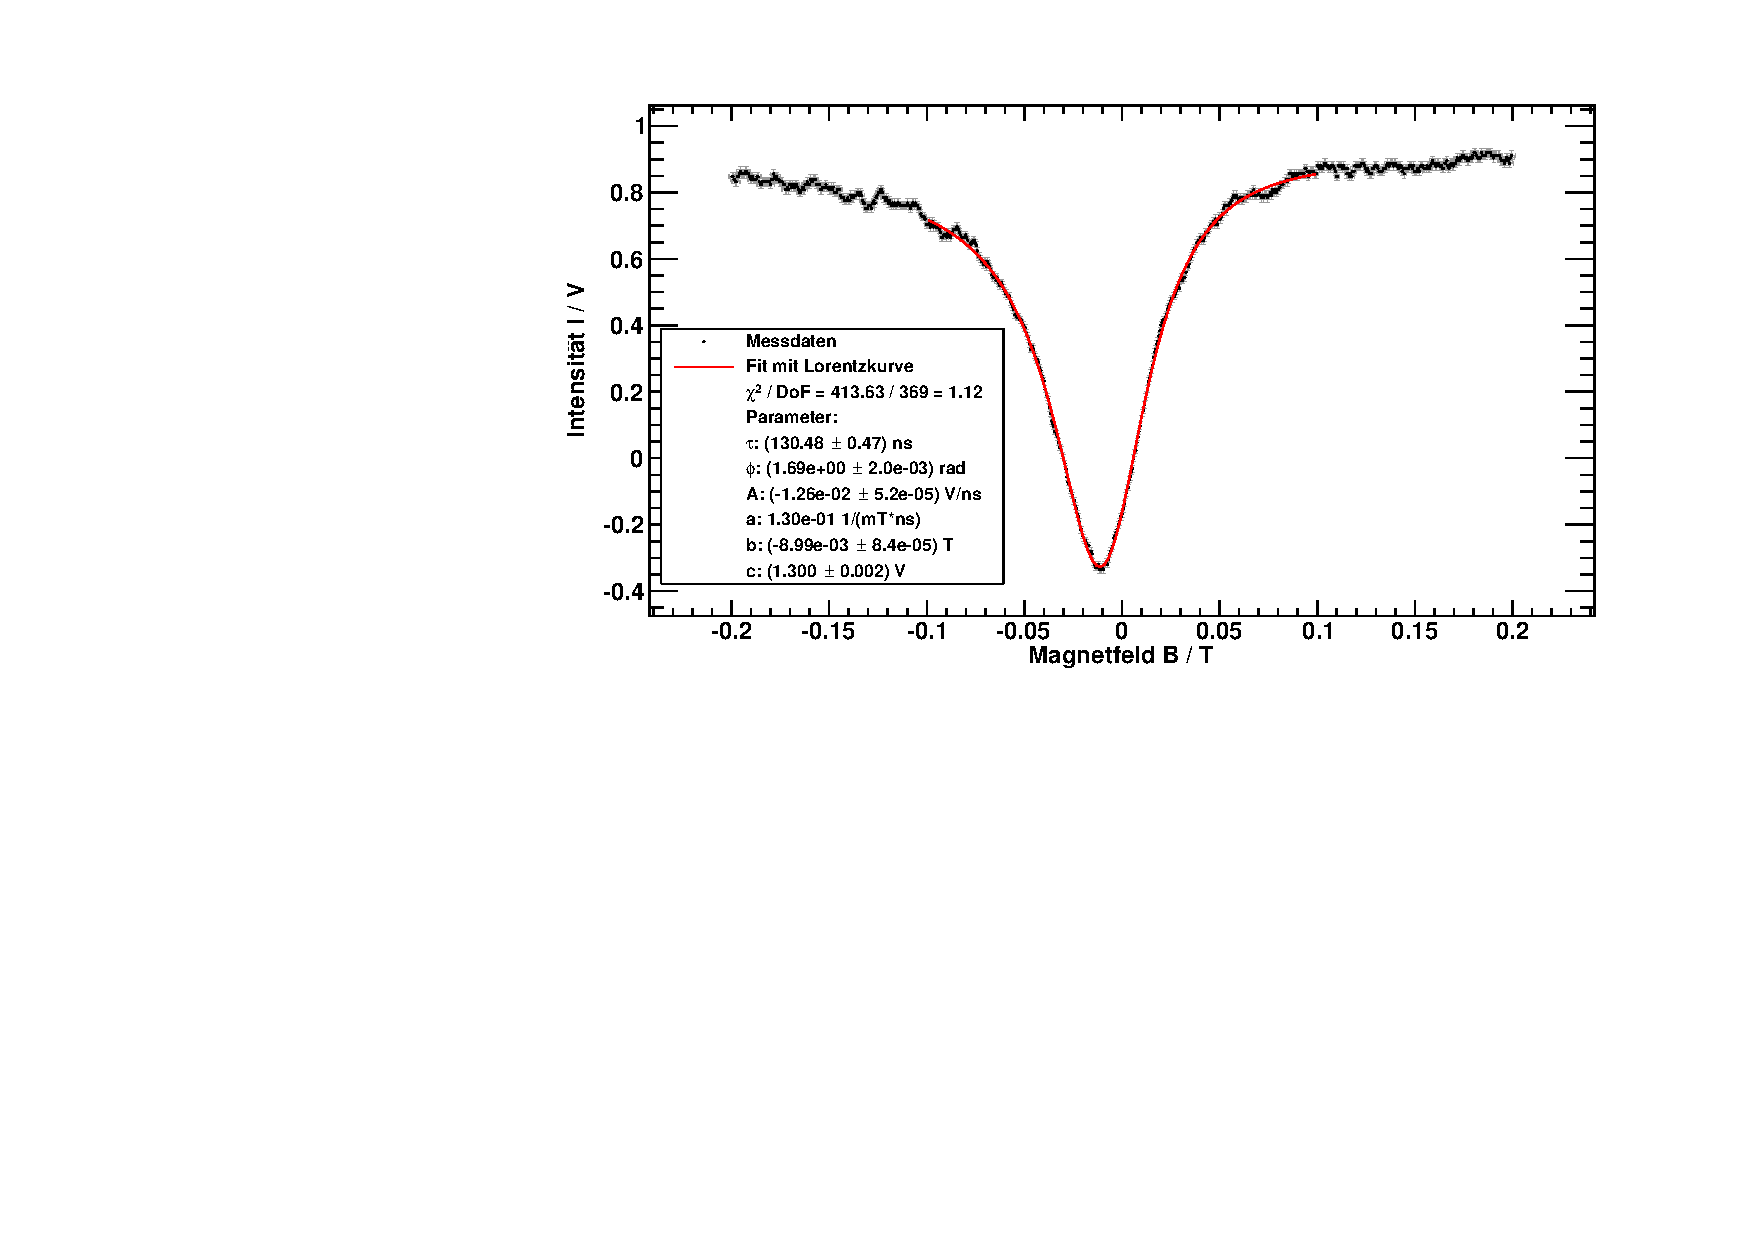
\includegraphics[width=\textwidth]{../img/fit_90_p05_6.pdf}
  \caption{Fit des Hanle-Signals mit Lorentzkurve. Hier exemplarisch für $T=5\,{}^\circ$C und $\Phi=90^\circ$.}
  \label{img:fit:lorentz:90}
\end{center}
\end{figure}
Die Fitergebnisse aller Messungen werden in Abschnitt \ref{subsub:fitresults} diskutiert.

\subsubsection{Fehler auf die Lebensdauer}
Der Fehler auf die Lebensdauer, den man aus dem Fit erhält, ist möglicherweise zu klein. Deshalb wurde für eine ausgewählte Temperatur ($T=5\,{}^\circ$C) 
die Messung bei $\Phi=0^\circ$ und $\Phi=90^\circ$ mehrmals ($N=10$) durchgeführt. Aus dem Mittelwert und der Standardabweichung wurde 
nun ein relativer Fehler auf $\tau$ berechnet. Man erhält:
\begin{equation}
  \label{eq:error:tau:0_90}
  \left( \frac{s_\tau}{\tau} \right)_{0^\circ} = 0.013 \qquad \left( \frac{s_\tau}{\tau} \right)_{90^\circ} = 0.011
\end{equation}
Für den Fehler auf die Lebensdauern bei $\Phi=90^\circ$ wurde aus den beiden Fehlern der Mittelwert gebildet.
\begin{equation}
  \label{eq:error:tau:45}
  \left( \frac{s_\tau}{\tau} \right)_{0^\circ} = 0.012
\end{equation}
\subsubsection{Fitergebnisse}
\label{subsub:fitresults}
Die Ergebnisse für die drei Winkel sind in \autoref{tab:phi:0}, \autoref{tab:phi:45} und \autoref{tab:phi:90} aufgelistet. Die Fehler der 
Lebensdauern sind wie oben beschrieben aus der Standardabweichung der Lebensdauern bei konstanter Temperatur bestimmt worden. Bei den Fehlern 
der Winkel wurde diese Korrektur nicht vorgenommen; hier wurden die Fehler aus den Fits verwendet. Die Lebensdauern werden in 
\ref{subsub:fittaus} gefittet.
\begin{table}[H]
\caption{Fitergebnisse f"ur $\Phi=0^\circ$.}
\begin{center}
\begin{tabular}{|c|c|c|c|c|}
  \hline
  $T$ / ${}^{\circ}$C & $\tau$ / ns & $s_{\tau}$ / ns & $\Phi$ / ${}^{\circ}$ & $s_{\Phi}$ / ${}^{\circ}$ \\ \hline
  23 & 124.9 & 1.6 & 0.648 & 0.032 \\ \hline
  19 & 122.1 & 1.5 & 0.906 & 0.029 \\ \hline
  14 & 122.9 & 1.5 & 0.041 & 0.025 \\ \hline
  10 & 116.1 & 1.5 & -0.447 & 0.019 \\ \hline
  7 & 122.9 & 1.5 & 0.219 & 0.020 \\ \hline
  5 & 116.6 & 1.5 & -0.056 & 0.139 \\ \hline
  3 & 111.7 & 1.4 & -0.238 & 0.020 \\ \hline
  0 & 110.4 & 1.4 & -0.288 & 0.020 \\ \hline
  -1 & 109.1 & 1.4 & -0.155 & 0.020 \\ \hline
  -3 & 104.2 & 1.3 & -0.538 & 0.025 \\ \hline
  -4 & 105.1 & 1.3 & -0.458 & 0.024 \\ \hline
  -7 & 102.2 & 1.3 & -0.476 & 0.029 \\ \hline
  -8 & 106.5 & 1.3 & -0.407 & 0.042 \\ \hline
\end{tabular}
\end{center}
\label{tab:phi:0}
\end{table}

\begin{table}[H]
\caption{Fitergebnisse f"ur $\varphi=45$}
\begin{center}
\begin{tabular}{|c|c|c|c|c|}
  \hline
  $T$ / ${}^{\circ}$C & $\tau$ / ns & $s_{\tau} / ns$ & $\varphi$ / ${}^{\circ}$ & $s_{\varphi}$ / ${}^{\circ}$ \\ \hline
  23 & 149.9 & 1.7 & 31.538 & 0.209 \\ \hline
  19 & 140.7 & 1.6 & 37.495 & 0.211 \\ \hline
  10 & 126.7 & 1.4 & 36.166 & 0.134 \\ \hline
  7 & 132.3 & 1.5 & 38.131 & 0.136 \\ \hline
  5 & 121.3 & 1.3 & 37.273 & 0.148 \\ \hline
  3 & 116.0 & 1.3 & 38.735 & 0.163 \\ \hline
  0 & 115.5 & 1.3 & 36.855 & 0.166 \\ \hline
  -1 & 120.6 & 1.3 & 35.438 & 0.156 \\ \hline
  -3 & 111.2 & 1.2 & 37.098 & 0.209 \\ \hline
  -4 & 111.2 & 1.2 & 35.342 & 0.222 \\ \hline
  -7 & 108.6 & 1.2 & 35.264 & 0.255 \\ \hline
  -8 & 104.6 & 1.2 & 38.696 & 0.331 \\ \hline
\end{tabular}
\end{center}
\label{tab:phi:45}
\end{table}

\begin{table}[H]
\caption{Fitergebnisse f"ur $\varphi=90$}
\begin{center}
\begin{tabular}{|c|c|c|c|c|}
  \hline
  $T$ / ${}^{\circ}$C & $\tau$ / ns & $s_{\tau} / ns$ & $\varphi$ / ${}^{\circ}$ & $s_{\varphi}$ / ${}^{\circ}$ \\ \hline
  23 & 160.5 & 1.7 & 88.197 & 0.095 \\ \hline
  19 & 164.0 & 1.8 & 89.482 & 0.087 \\ \hline
  10 & 134.6 & 1.4 & 95.995 & 0.049 \\ \hline
  7 & 134.8 & 1.4 & 95.089 & 0.053 \\ \hline
  5 & 131.0 & 1.4 & 96.695 & 0.499 \\ \hline
  3 & 123.9 & 1.3 & 97.930 & 0.054 \\ \hline
  0 & 126.2 & 1.4 & 97.914 & 0.054 \\ \hline
  -1 & 119.0 & 1.3 & 89.235 & 0.053 \\ \hline
  -3 & 116.3 & 1.2 & 89.605 & 0.059 \\ \hline
  -4 & 113.5 & 1.2 & 96.982 & 0.068 \\ \hline
  -7 & 110.3 & 1.2 & 97.656 & 0.076 \\ \hline
  -8 & 109.4 & 1.2 & 98.378 & 0.086 \\ \hline
\end{tabular}
\end{center}
\label{tab:phi:90}
\end{table}


Mann kann für jeden Winkel den Mittelwert aus den gefitteten Winkeln bestimmen (\autoref{tab:avgphis}). Der Fehler berechnet sich aus der 
Standardabweichung, dividiert durch die Wurzel der Anzahl der Messungen. Man erkennt, dass für die $0^\circ$-Einstellung das Ergebnis gut mit dem 
gewünschten Wert übereinstimmt. Die $90^\circ$-Einstellung liegt ca. 4 Standardabweichungen daneben. Bei der $45^\circ$-Einstellung liegt der 
gefittete Wert weit neben dem Gewünschten. Dies liegt daran, dass der Abstand zwischen $0^\circ$- und $90^\circ$-Einstellung auf der Winkelskala 
des Polarisationsfilters nicht genau $90^\circ$ betrug und trotzdem die $45^\circ$-Einstellung genau $45^\circ$ unterhalb der $90^\circ$-Einstellung 
gewählt wurde (siehe \ref{sub:calibration}). Für die Bestimmung der Lebensdauern spielt dies hier jedoch keine Rolle, da der Winkel beim Fit 
nicht festgelegt wurde.
\begin{table}[H]
\caption{Theoretischer und gefitteter Winkel der drei Einstellungen am Aufbau.}
\begin{center}
\begin{tabular}{|c|c|c|}
  \hline
  $\Phi$ / ${}^{\circ}$ & $\Phi_\text{fit}$ / ${}^{\circ}$ & $s_{\Phi_\text{fit}}$ / ${}^{\circ}$ \\ \hline
  0 & -0.10 & 0.12 \\ \hline
  45 & 36.53 & 0.59 \\ \hline
  90 & 94.43 & 1.15 \\ \hline
\end{tabular}
\end{center}
\label{tab:avgphis}
\end{table}


\subsection{Extrapolation der mittleren Lebensdauern auf  \texorpdfstring{0\,Pa}{0 Pa}}
Um nun die richtige Lebensdauer zu bestimmen, müssen die gefitteten Lebensdauern über dem Dampfdruck des Quecksilbers aufgetragen werden und auf 
0\,Pa extrapoliert werden.
\subsubsection{Berechnung des Dampfdrucks aus der Temperatur}
Der Dampfdruck wird mit \autoref{eq:vaporpress} berechnet (\autoref{tab:pressure}). Der Fehler folgt aus der Gauß'schen Fehlerfortpflanzung.
Dabei wird die oben angegebene Kovarianzmatrix (\autoref{eq:cov}) benutzt.
\begin{equation}
\begin{split}
  & f = f(x_1, \ldots, x_n) \\
  & s_f^2 = \sum_{i, j}^n \left( \frac{\partial f}{\partial x_i} \right) \left( \frac{\partial f}{\partial x_j} \right) \cov(x_i, x_j)
\end{split}
\end{equation}
Dabei wurde ein Fehler von 2\,K auf die Temperatur angenommen.
\begin{table}[H]
\caption{Dampfdruck von Quecksilber bei verschiedenen Temperaturen.}
\begin{center}
\begin{tabular}{|c|c|c|}
  \hline
  $T$ / ${}^{\circ}$C & $p$ / mPa & $s_p$ / mPa \\ \hline
  23 & 221 & 37 \\ \hline
  19 & 157 & 27 \\ \hline
  14 & 101 & 18 \\ \hline
  10 & 70 & 13 \\ \hline
  7 & 53 & 10 \\ \hline
  5 & 44 & 8 \\ \hline
  3 & 36 & 7 \\ \hline
  0 & 27 & 5 \\ \hline
  -1 & 24 & 5 \\ \hline
  -3 & 20 & 4 \\ \hline
  -4 & 18 & 4 \\ \hline
  -7 & 13 & 3 \\ \hline
  -8 & 12 & 3 \\ \hline
\end{tabular}
\end{center}
\label{tab:pressure}
\end{table}

\subsubsection{Bestimmung der Lebensdauer}
\label{subsub:fittaus}
Die Lebensdauern bei den drei Winkeleinstellungen sind in \autoref{img:taus:00}, \autoref{img:taus:45} und \autoref{img:taus:90} über 
dem oben berechneten Dampfdruck aufgetragen. 

\begin{figure}[H]
\begin{center}
  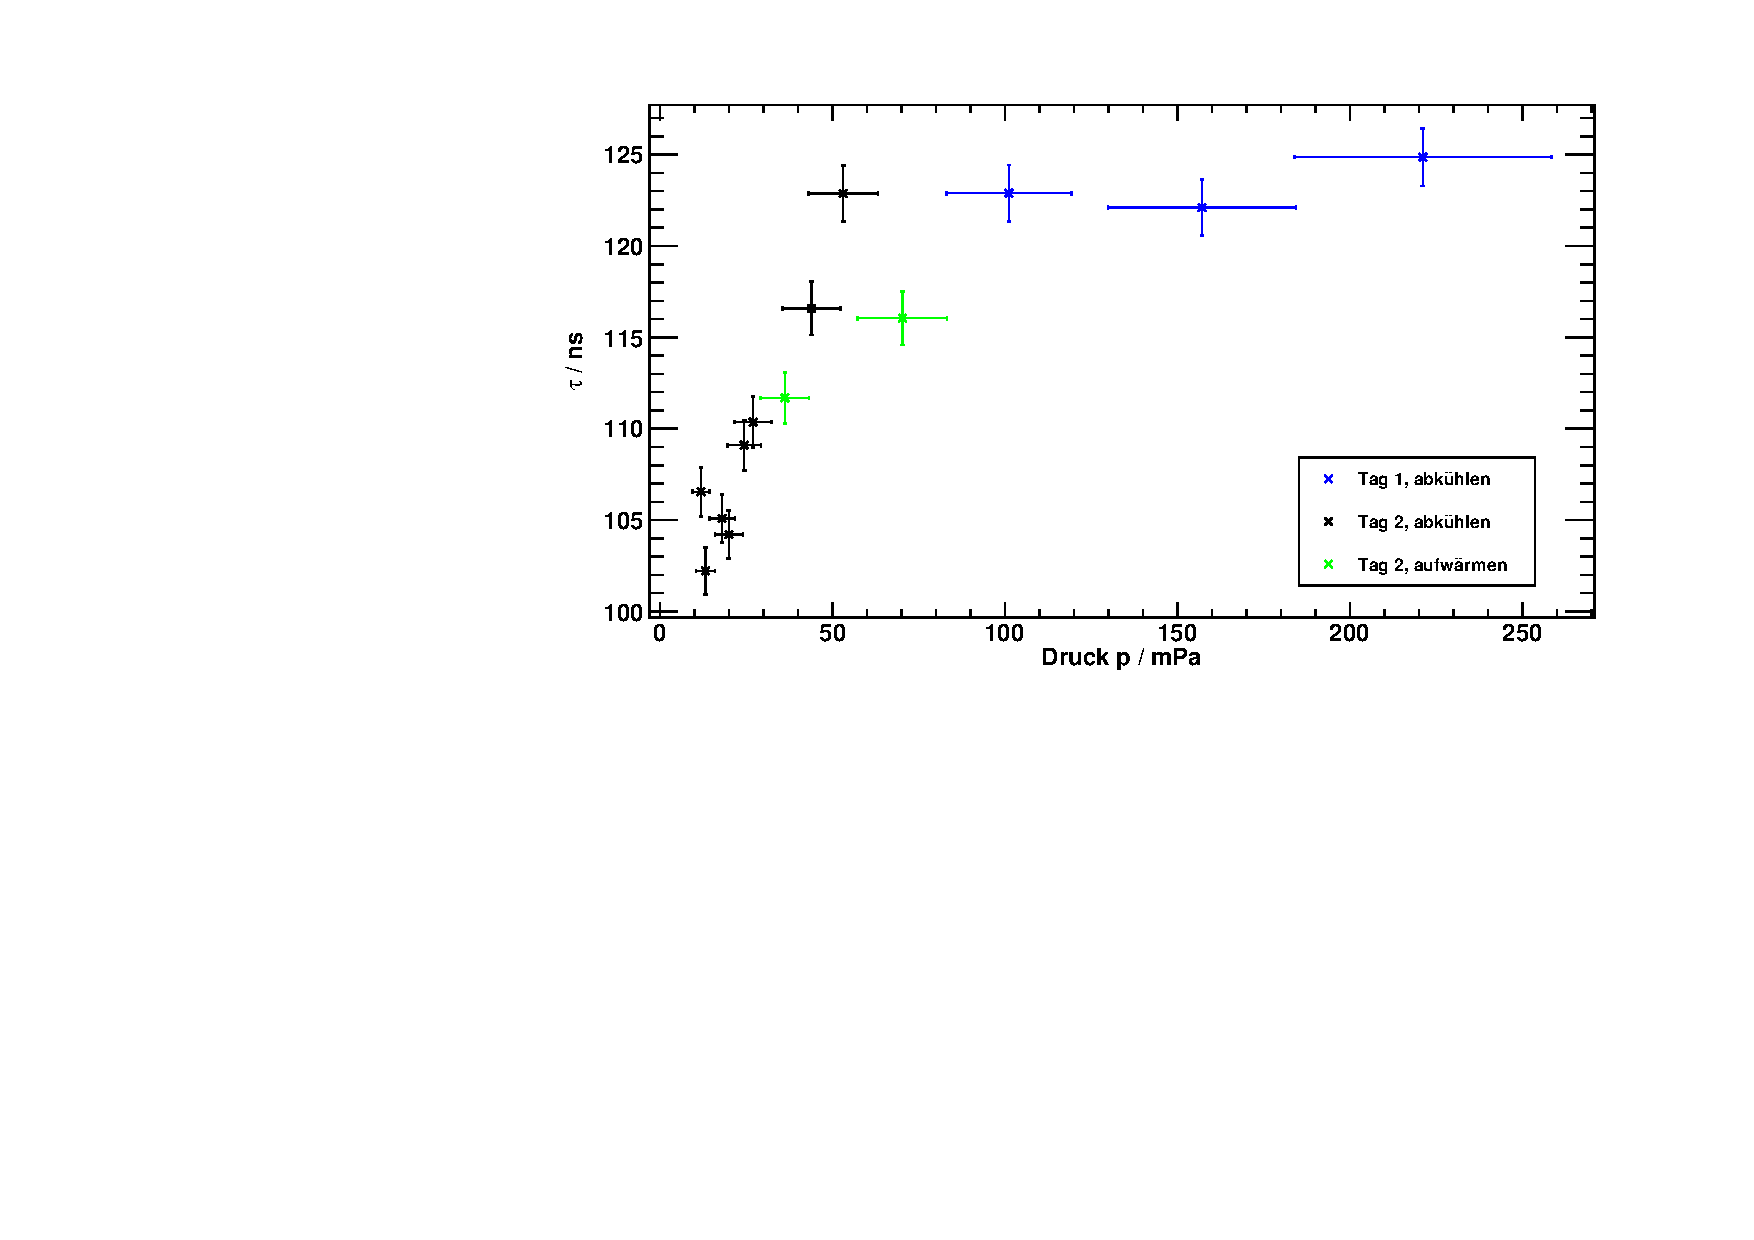
\includegraphics[width=\textwidth]{../img/taus_00.pdf}
  \caption{caption}
  \label{img:taus:00}
\end{center}
\end{figure}

\begin{figure}[H]
\begin{center}
  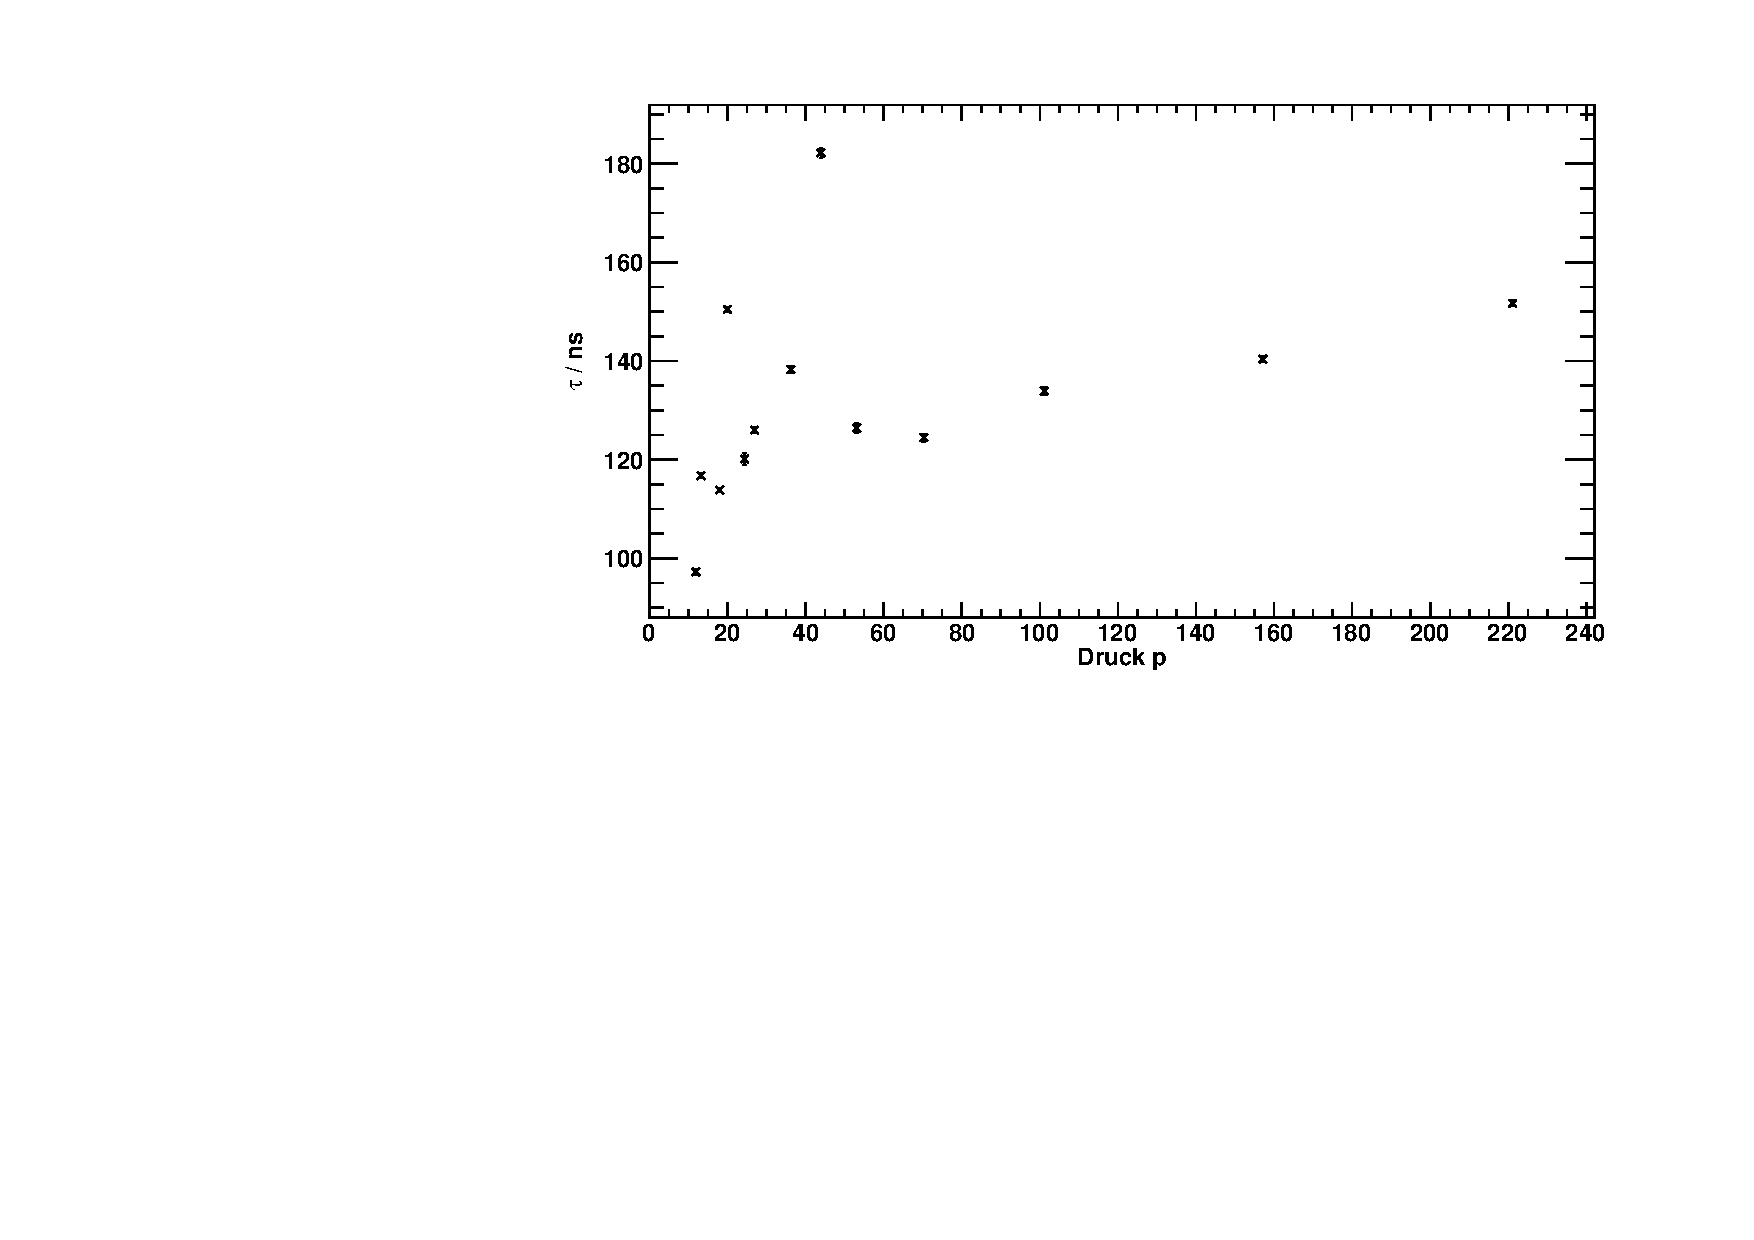
\includegraphics[width=\textwidth]{../img/taus_45.pdf}
  \caption{caption}
  \label{img:taus:45}
\end{center}
\end{figure}

\begin{figure}[H]
\begin{center}
  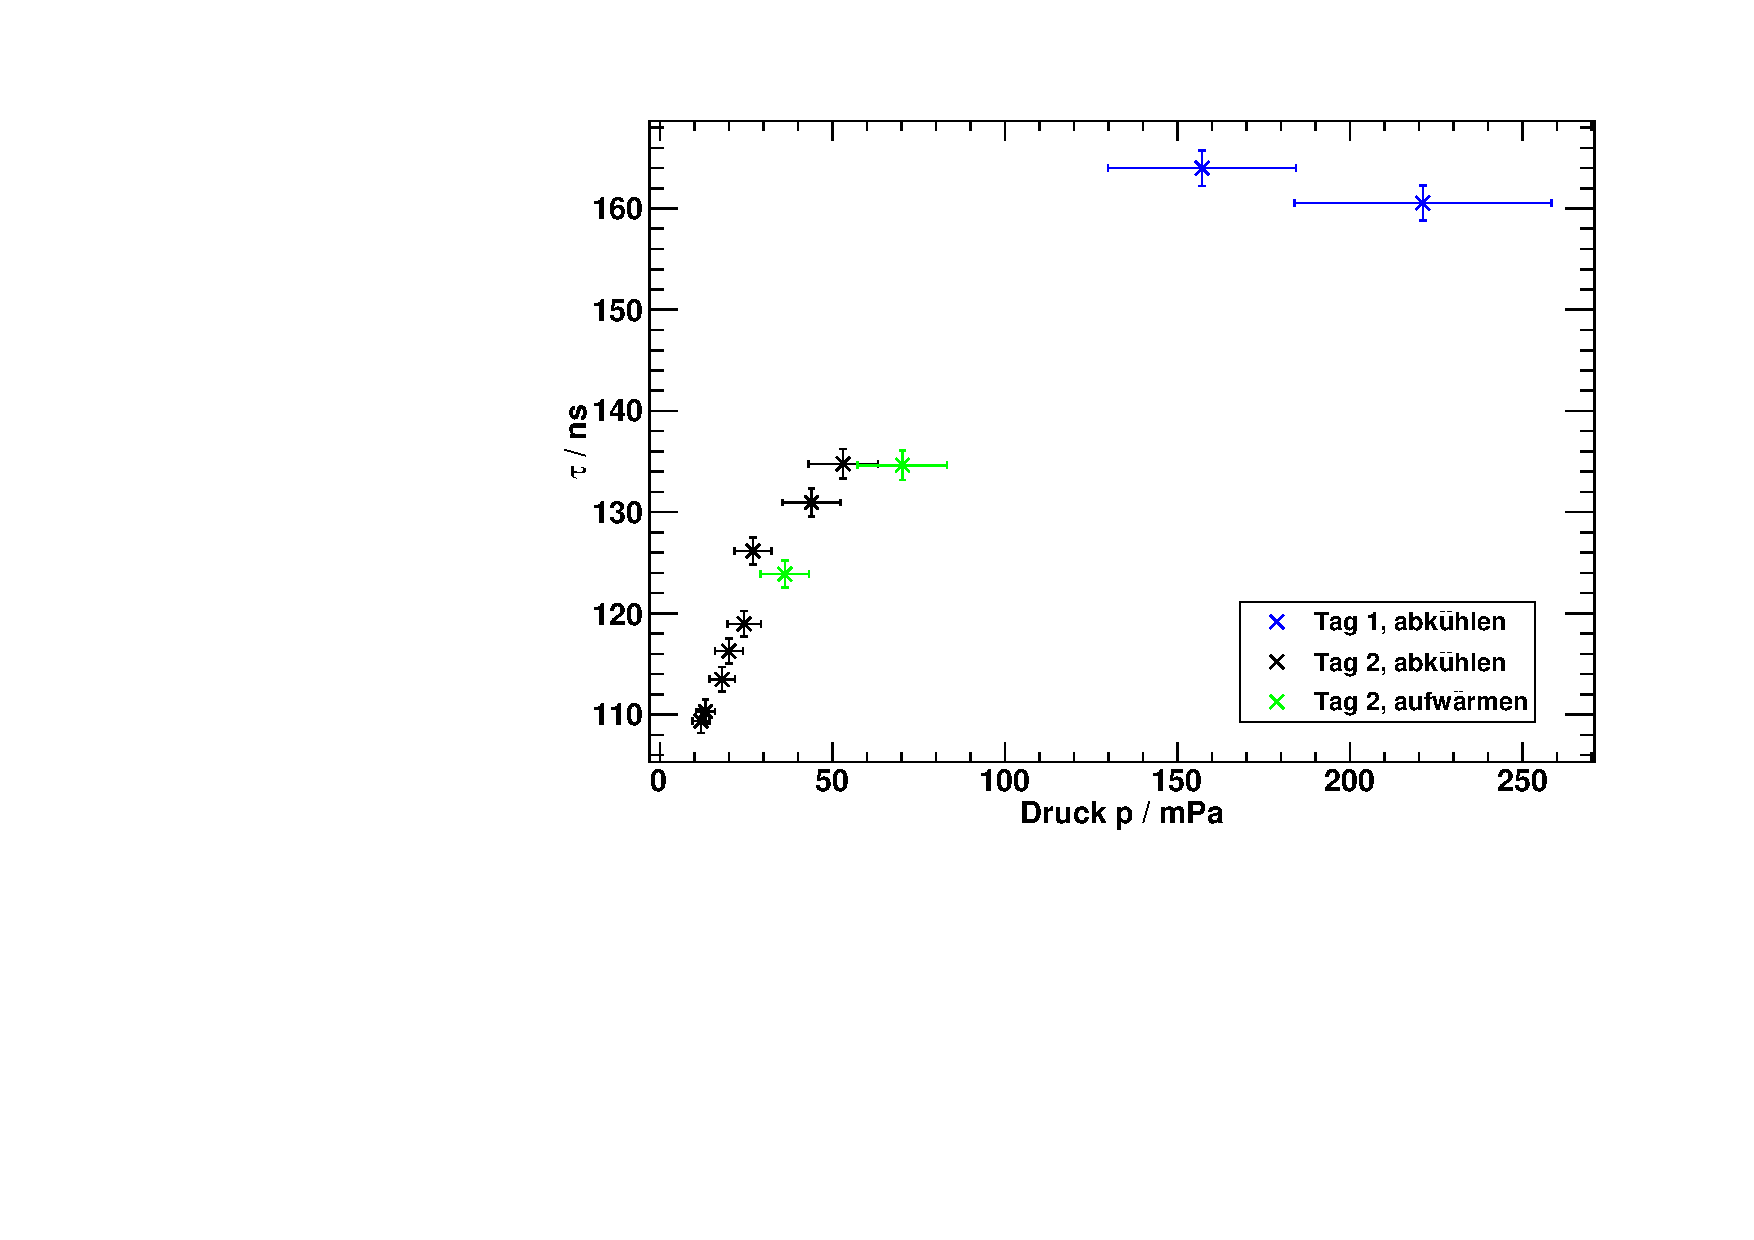
\includegraphics[width=\textwidth]{../img/taus_90.pdf}
  \caption{caption}
  \label{img:taus:90}
\end{center}
\end{figure}

Man sieht, dass die Werte vom ersten Tag nicht in den linearen Zusammenhang passen. Außerdem 
sieht man in \autoref{img:TI}, dass die Temperaturen des ersten Tages nicht mit denen des zweiten Tages konsistent sind. Dies sollte zwar kein 
Problem darstellen, falls die richtige Temperatur gemessen wurde, könnte aber trotzdem auf ein Problem hindeuten. Deshalb wurden die Werte des 
ersten Tages bei der folgenden Extrapolation nicht mit berücksichtigt. \\
Die Lebensdauern werden nun mit Geraden gefittet (\autoref{img:taus:day2:00}, \autoref{img:taus:day2:45}, \autoref{img:taus:day2:90}).
\begin{equation}
  \tau(p) = \tau_0 + m \cdot p
\end{equation}
Der Achsenabschnitt $\tau_0$ liefert die von dem Effekt des \emph{Coherence Narrowing} bereinigte Lebensdauer.

\begin{figure}[H]
\begin{center}
  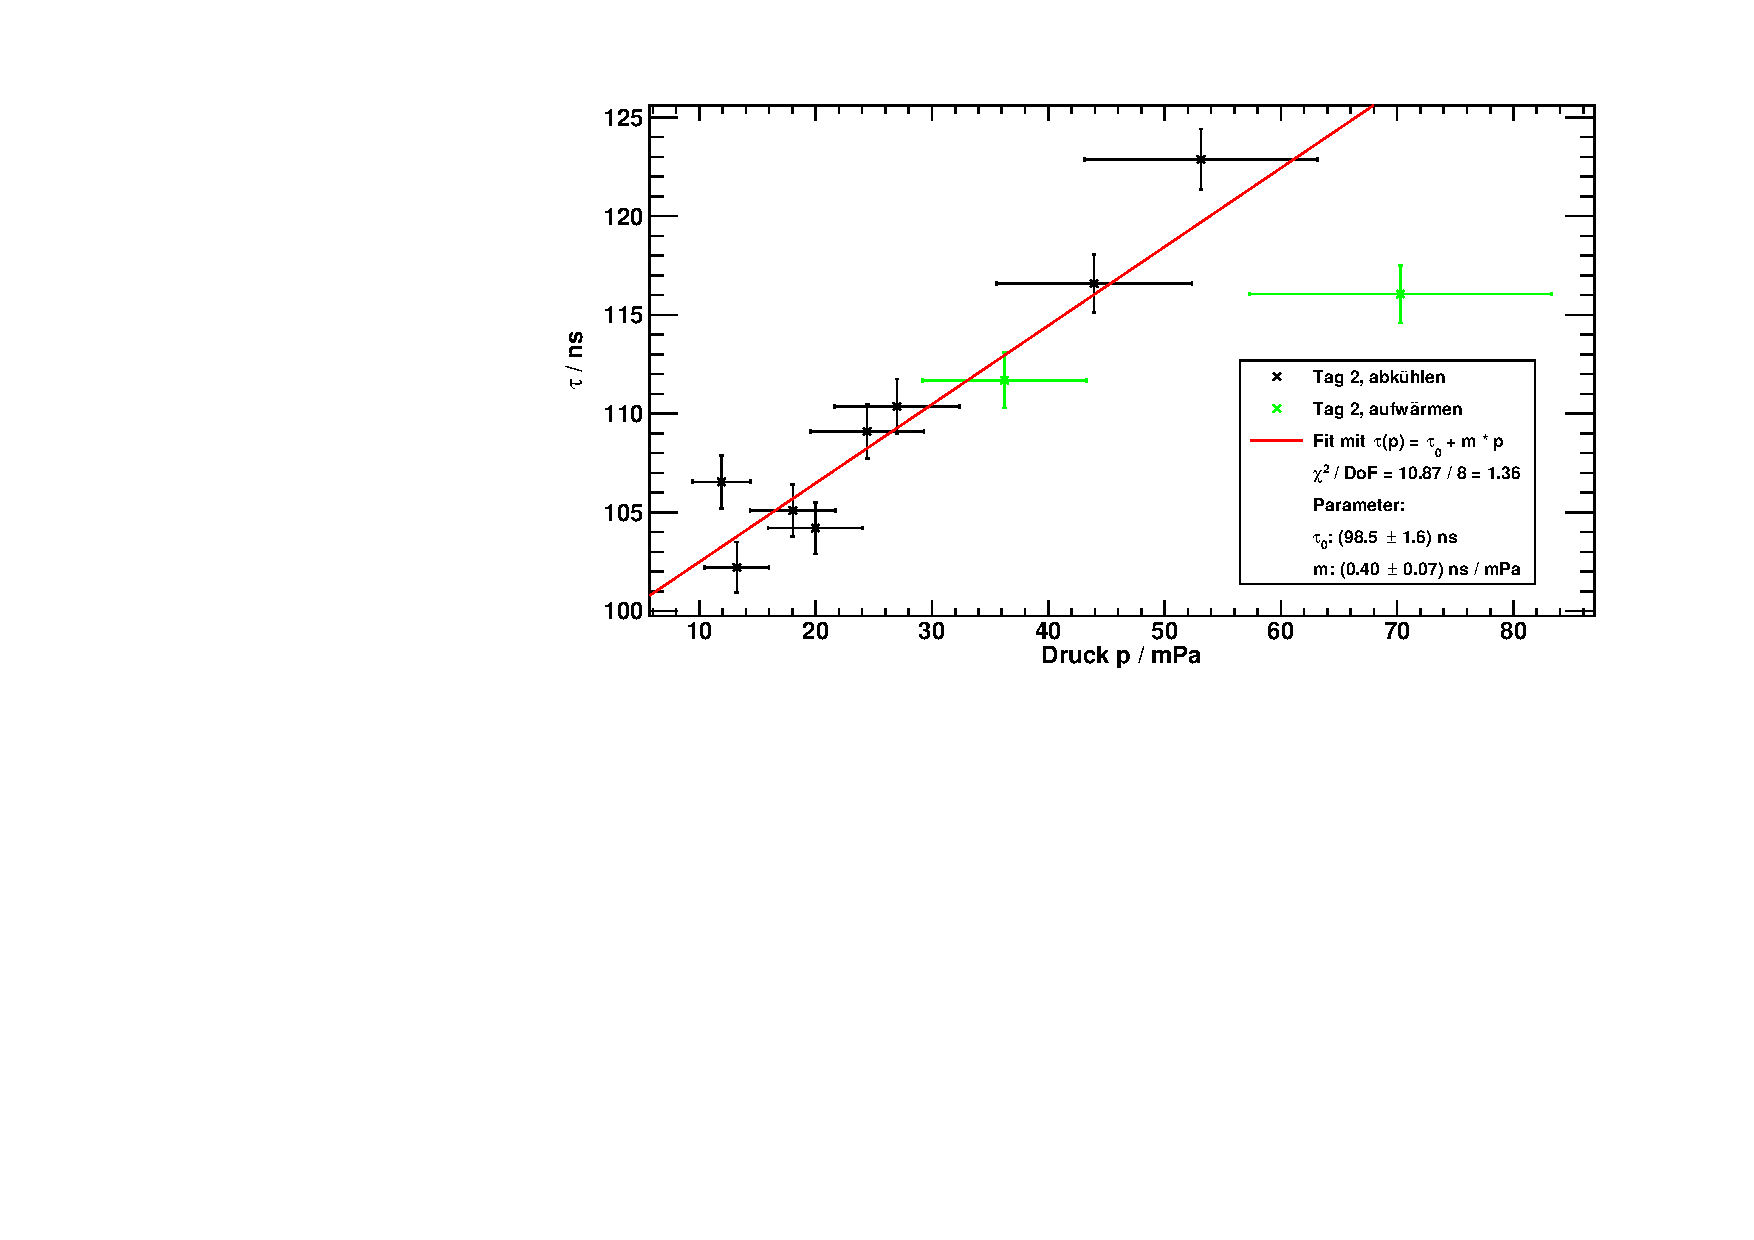
\includegraphics[width=\textwidth]{../img/taus_00_day2.pdf}
  \caption{caption}
  \label{img:taus:day2:00}
\end{center}
\end{figure}

\begin{figure}[H]
\begin{center}
  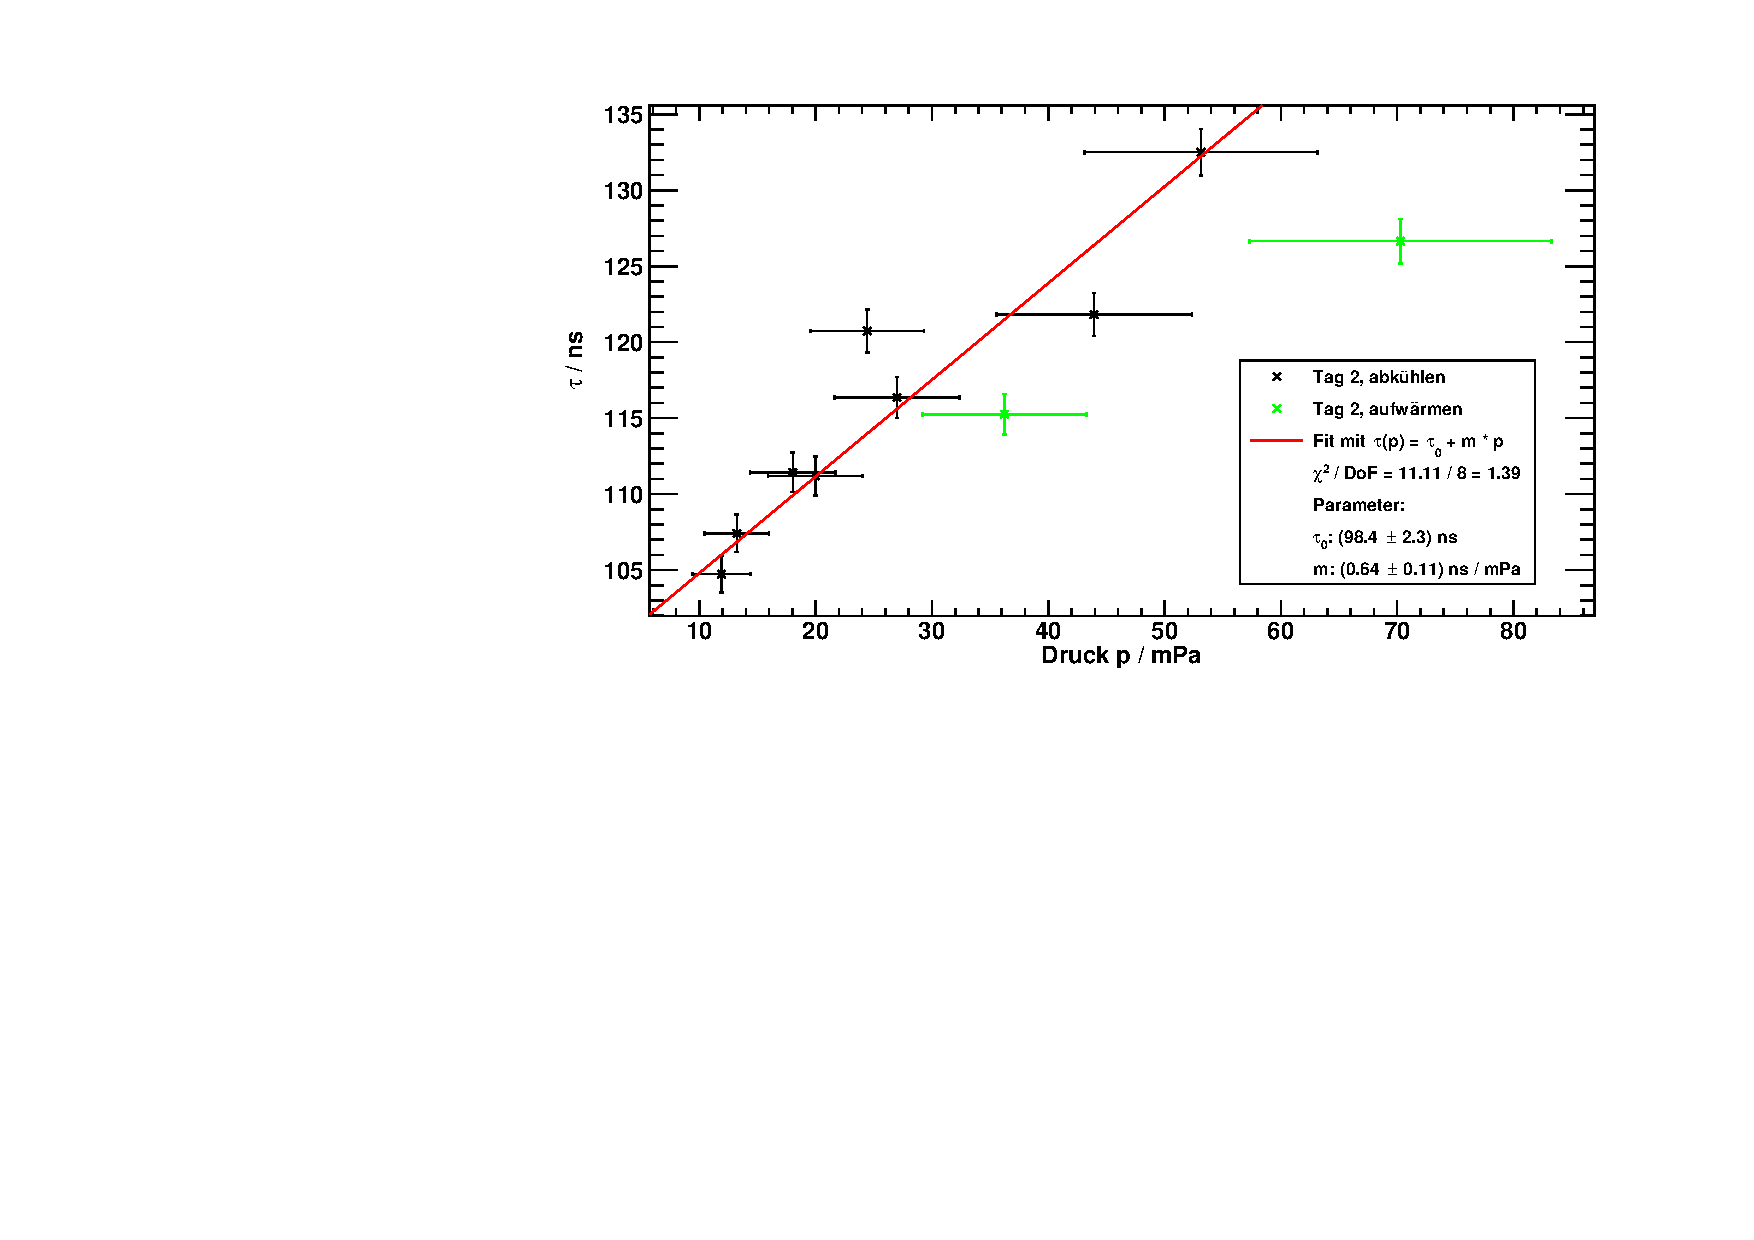
\includegraphics[width=\textwidth]{../img/taus_45_day2.pdf}
  \caption{caption}
  \label{img:taus:day2:45}
\end{center}
\end{figure}

\begin{figure}[H]
\begin{center}
  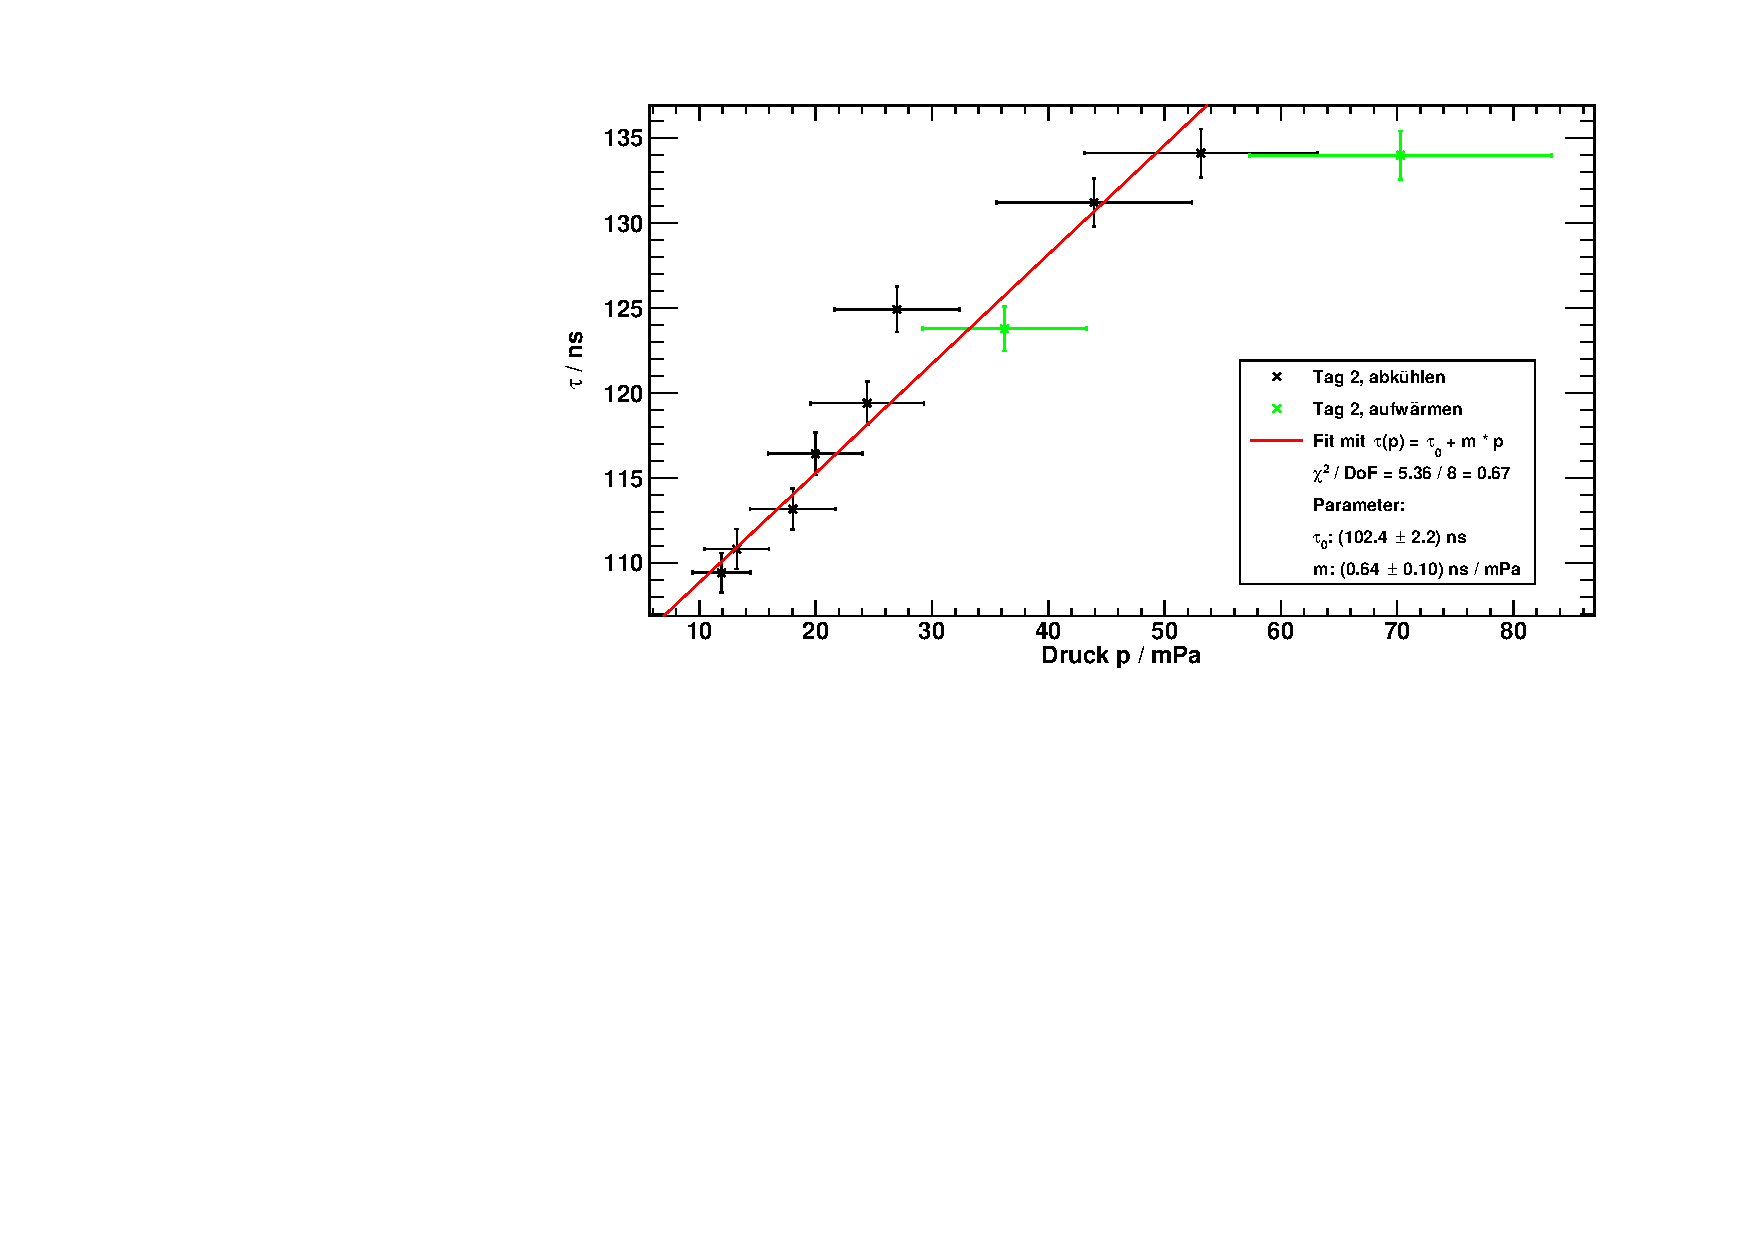
\includegraphics[width=\textwidth]{../img/taus_90_day2.pdf}
  \caption{caption}
  \label{img:taus:day2:90}
\end{center}
\end{figure}

\begin{table}[H]
\caption{Extrapolierte mittlere Lebensdauern bei verschiedenen Winkeleinstellungen.}
\begin{center}
\begin{tabular}{|c|c|c|}
  \hline
  $\Phi$ / ${}^{\circ}$ & $\tau$ / ns & $s_{\tau}$ / ns \\ \hline
  0 & 98.5 & 1.6 \\ \hline
  45 & 98.4 & 2.3 \\ \hline
  90 & 102.4 & 2.2 \\ \hline
\end{tabular}
\end{center}
\label{tab:tau:final}
\end{table}

